\textcolor{Mahogany}{Webbsidan består framför allt av olika problem som med hjälp av titel samt varsin tillhörande ikon listas i ett rutnät på webbplatsens ''Problem''-sida. Klickar man på ett av problemen så kommer man vidare till en mer detaljerad vy med en kort beskrivande text följt av en länk till det fullständiga problemet. I många fall bifogas även en tillhörande Google-presentation, som är tänkt att underlätta utförandet.}

\textcolor{Mahogany}{Webbplatsen har även en startsida där besökaren ges en introducerande text om webbplatsens syfte och innehåll samt att man via ett enkelt knapptryck lätt tar sig vidare till problemen. Dessa kommer man givetvis också åt via menyn, skillnaden är att vi vill fånga uppmärksamheten på ett mer välkomnande sätt för den som besöker webbplatsen för första gången genom att ha en knapp över en bild som illustrerar några av våra problem.}

\textcolor{Mahogany}{Till sist så inkluderas sidan ''Om oss'', som beskriver projektets arbete. Webbplatsen visas i figurerna \ref{fig:w1}, \ref{fig:w2}, \ref{fig:w3} respektive \ref{fig:w4}.}

\begin{figure}
\centering
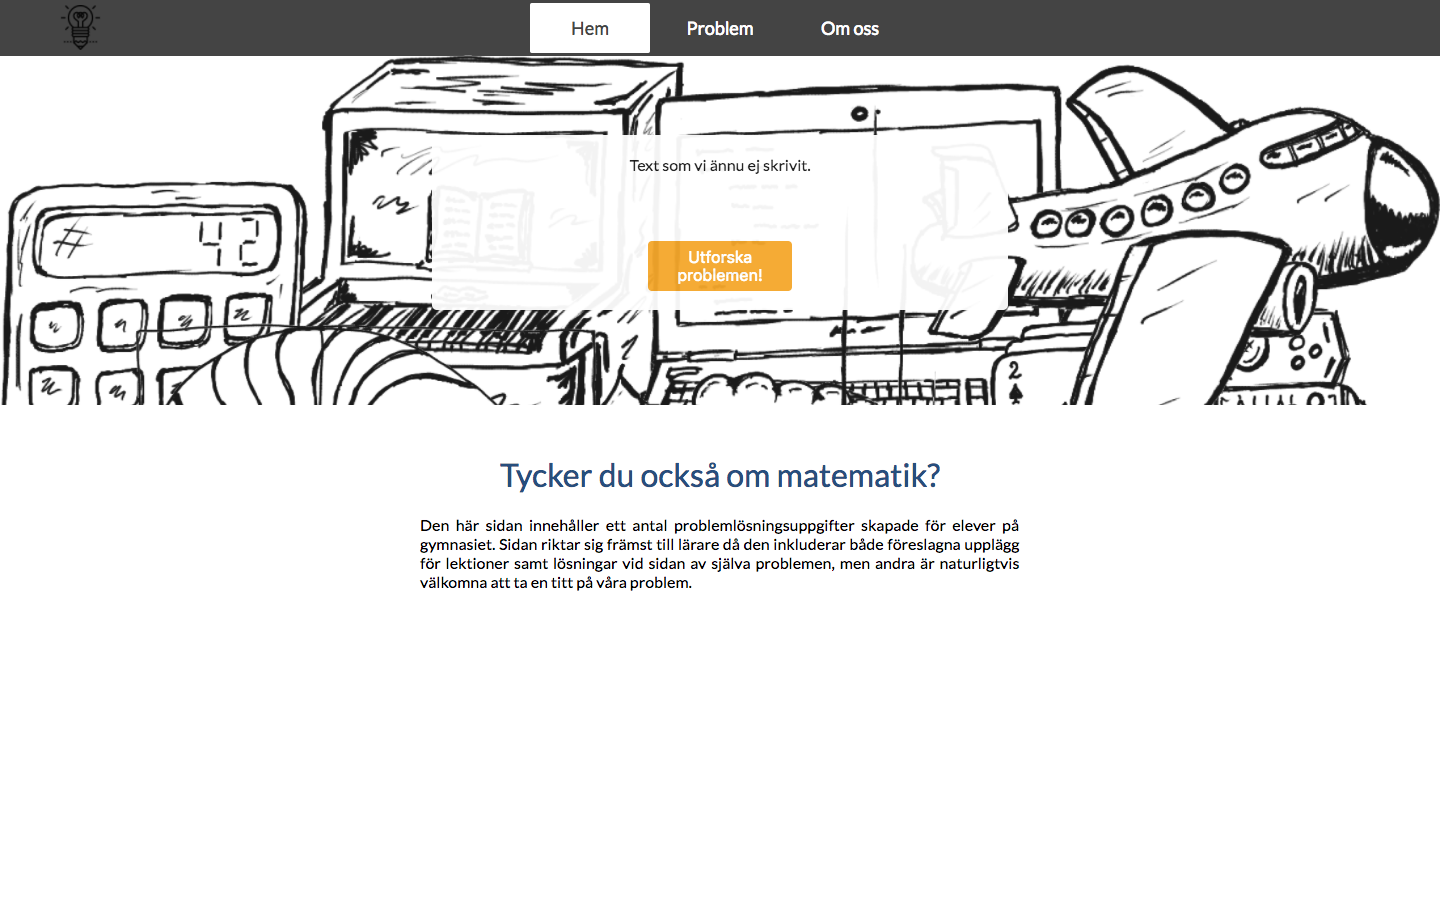
\includegraphics[width=0.8\textwidth]{Figures/Webbplatsen/Webbplats-startsida.png}
\caption{\textsl{Webbplatsens startsida}}
\label{fig:w1}
\end{figure}

\begin{figure}
\centering
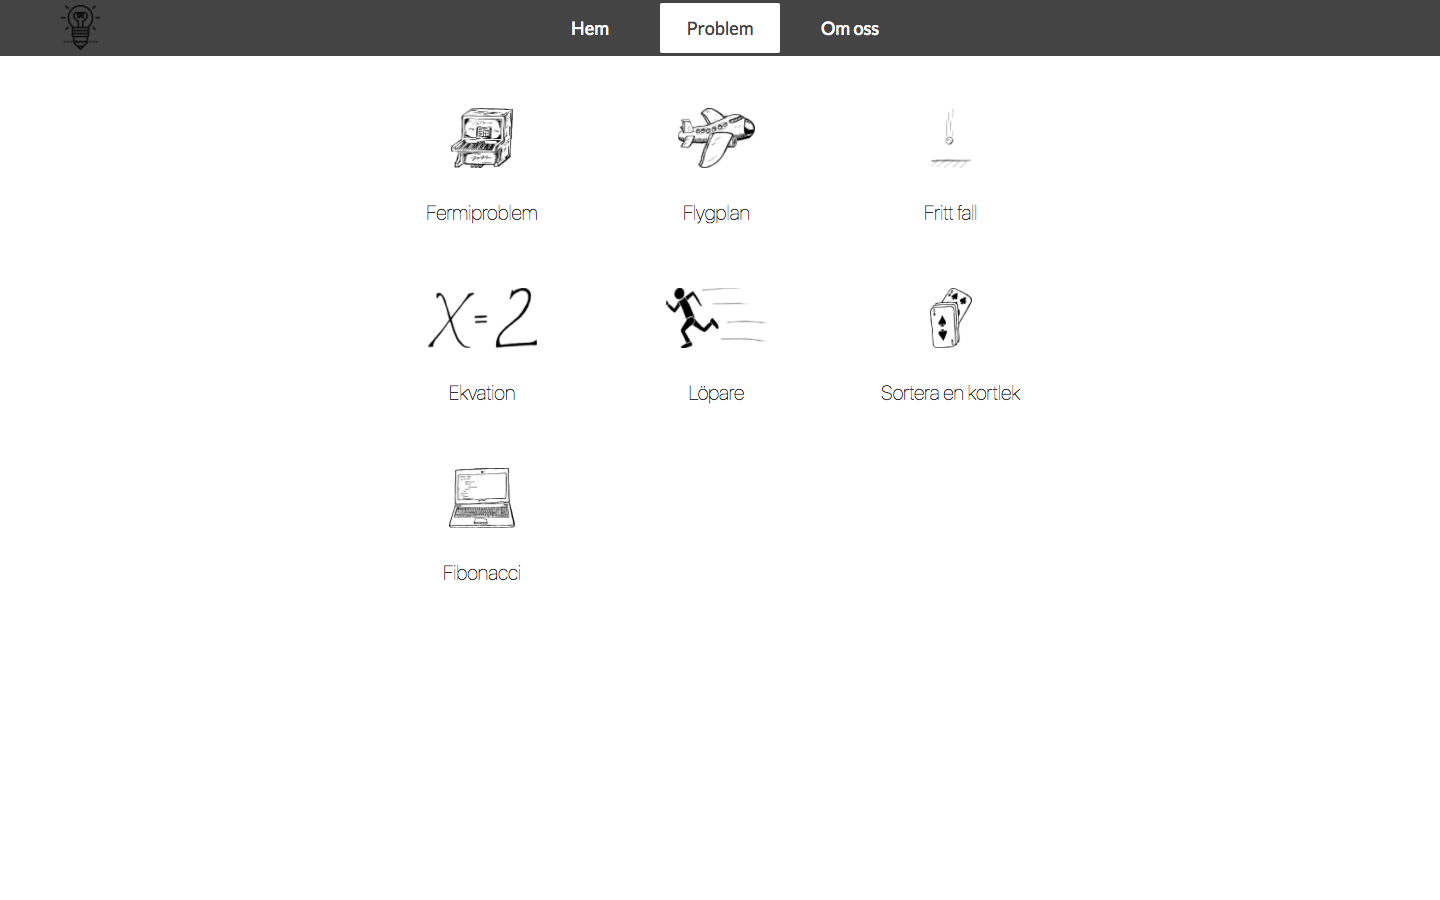
\includegraphics[width=0.8\textwidth]{Figures/Webbplatsen/Webbplats-problemlista.png}
\caption{\textsl{Webbplatsens problemsida}}
\label{fig:w2}
\end{figure}

\begin{figure}
\centering
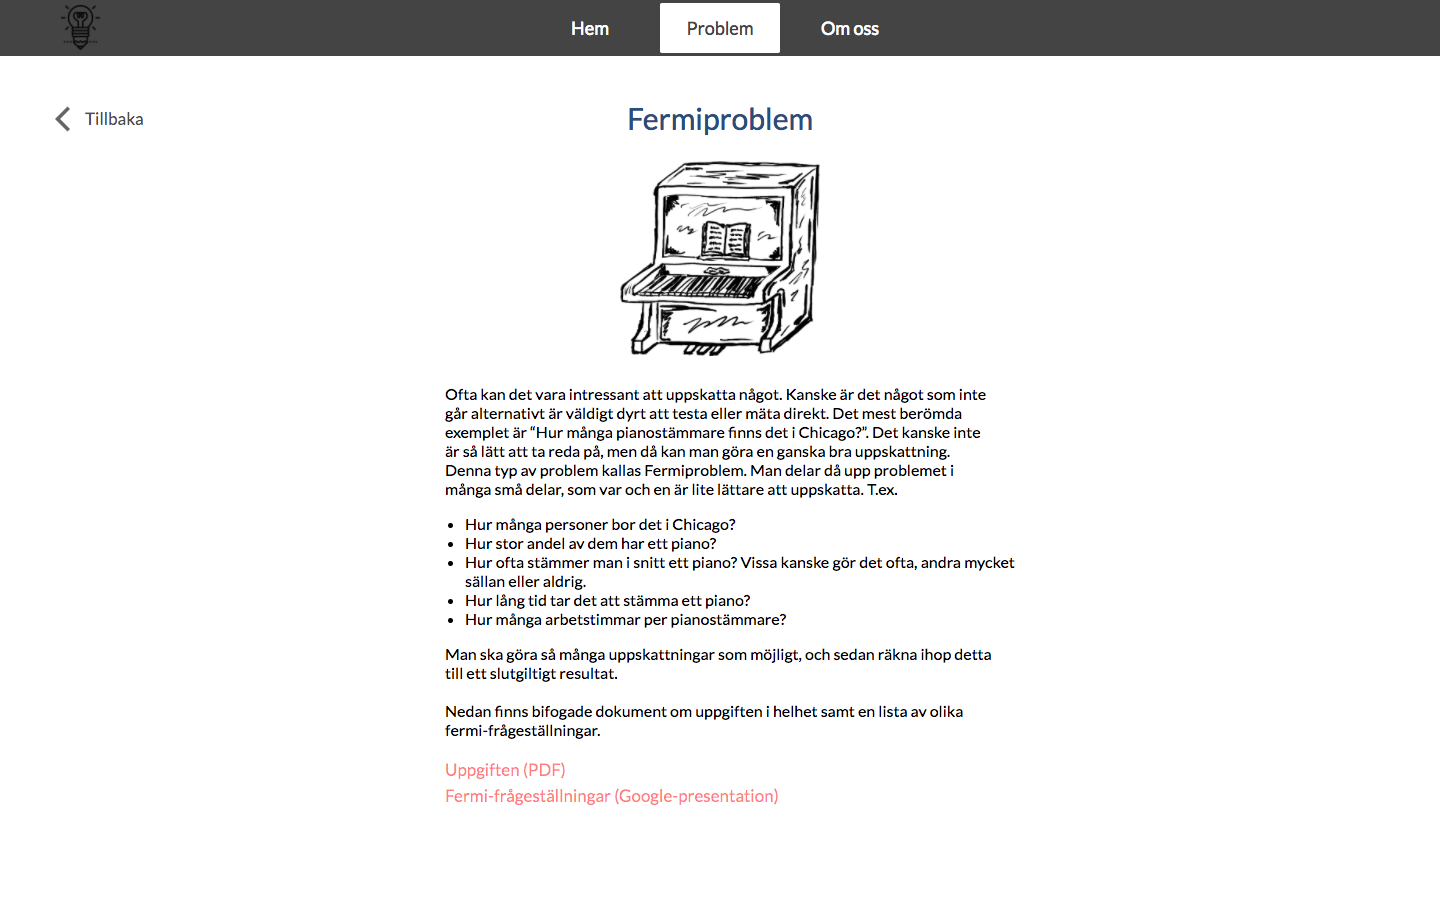
\includegraphics[width=0.8\textwidth]{Figures/Webbplatsen/Webbplats-problemvy.png}
\caption{\textsl{Webbplatsens problemvy}}
\label{fig:w3}
\end{figure}

\begin{figure}
\centering
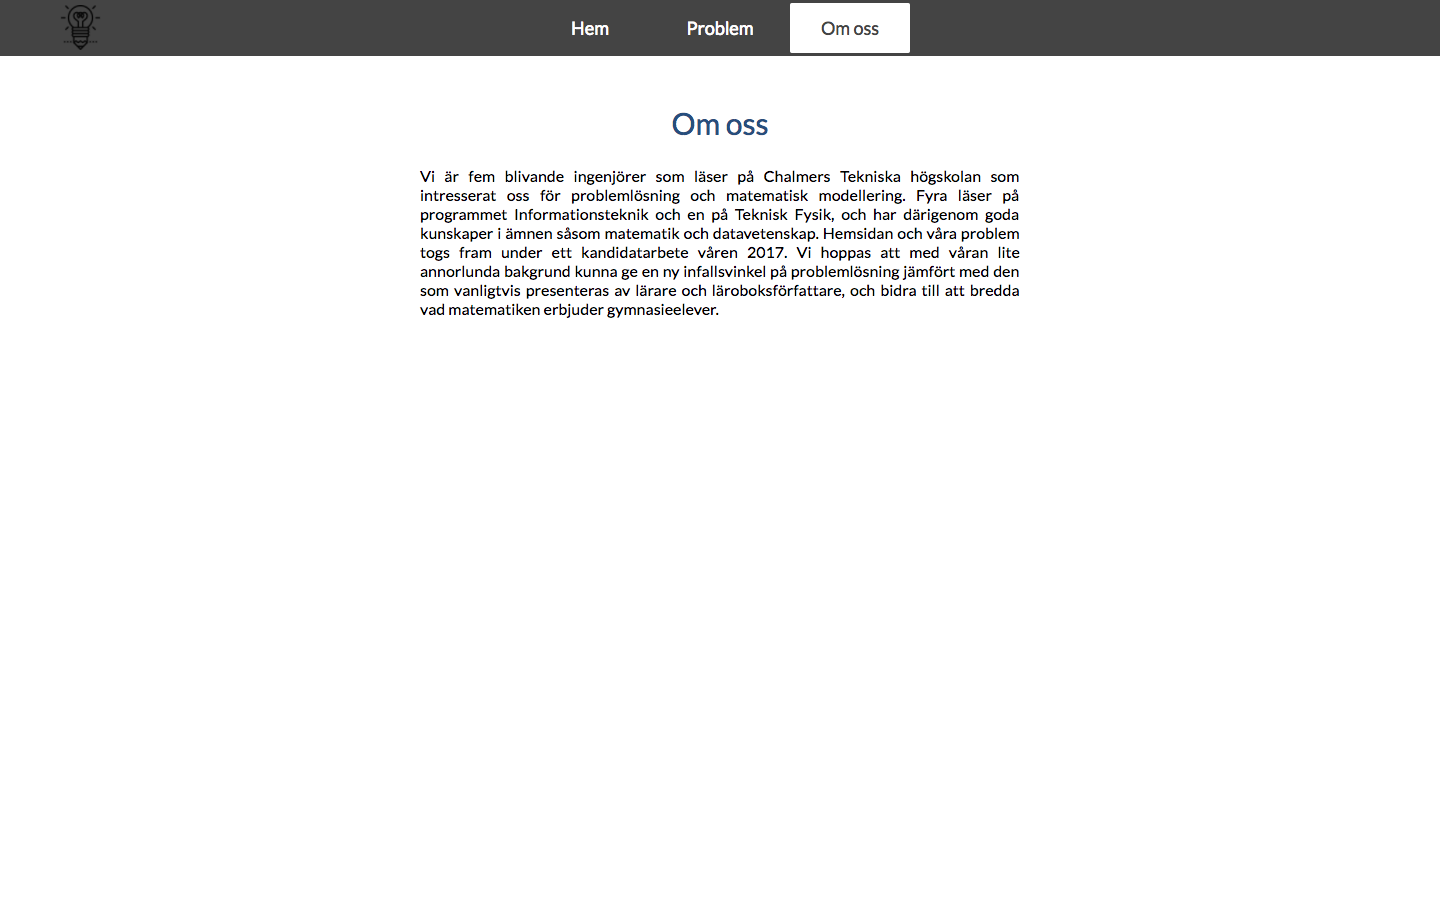
\includegraphics[width=0.8\textwidth]{Figures/Webbplatsen/Webbplats-omoss.png}
\caption{\textsl{Webbplatsens ''Om oss''-sida}}
\label{fig:w4}
\end{figure}
